\documentclass[11pt]{article}

\usepackage{graphicx,amsmath,amssymb,pgfplots}

\usepackage[letterpaper, margin=1in]{geometry}



\begin{document}

\title{Your Title Here}

\author{Your Name}

\date{Date}

\maketitle

\section{Introduction}  PUT CONTENT HERE; PERHAPS CITE SOMETHING \cite{einstein}

% HOW TO INCLUDE A FIGURE FROM AN IMAGE FILE:
\begin{figure}[ht]
\centering
\includegraphics[width=0.3\textwidth]{stencil.png}  % put image "stencil.png" in current directory
\caption{If there is no image above then that is because \texttt{stencil.png} is not on the path.}
\label{fig:stencil}
\end{figure}

\section{Continuum Model [or Continuum Problem]}  PUT CONTENT HERE; PERHAPS CITE SOMETHING \cite{ockendonetal}


\section{Numerical Scheme(s)}  PUT CONTENT HERE; PERHAPS CITE SOMETHING \cite{leveque}; REFER TO FIGURES BY LABELS, such as Figure \ref{fig:vcycle}.


% HERE IS A FIGURE GENERATED BY TIKZ COMMANDS
\begin{figure}[ht]
\centering
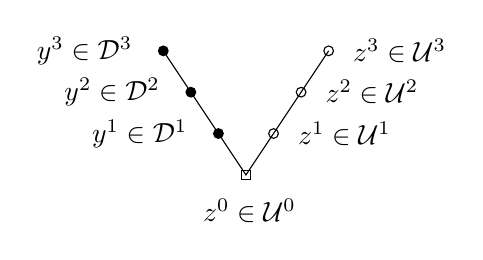
\begin{tikzpicture}[scale=0.7]
  \pgfmathsetmacro\hstep{0.5}
  \pgfmathsetmacro\vstep{0.75}
  \pgfmathsetmacro\ceps{0.08}   % size of square for coarse grid

% V-cycle with MCD down-obstacle and up-obstacle annotations
  \draw[black,thin] (-\hstep,3*\vstep) -- (0.0,2*\vstep) -- (\hstep,\vstep) --  (2*\hstep,0.0)
                    -- (3*\hstep,\vstep) -- (4*\hstep,2*\vstep) -- (5*\hstep,3*\vstep);
  \filldraw (-\hstep,3*\vstep) node[xshift=-10mm] {$y^3 \in \mathcal{D}^3$} circle (2.5pt);
  \filldraw (0.0,2*\vstep) node[xshift=-10mm] {$y^2 \in \mathcal{D}^2$} circle (2.5pt);
  \filldraw (\hstep,\vstep) node[xshift=-10mm] {$y^1 \in \mathcal{D}^1$} circle (2.5pt);
  \draw     (2*\hstep-\ceps,-\ceps) node[xshift=1mm,yshift=-4mm] {$z^0 \in \mathcal{U}^0$} rectangle (2*\hstep+\ceps,+\ceps);
  \draw     (3*\hstep,\vstep) node[xshift=9mm] {$z^1 \in \mathcal{U}^1$} circle (2.5pt);
  \draw     (4*\hstep,2*\vstep) node[xshift=9mm] {$z^2 \in \mathcal{U}^2$} circle (2.5pt);
  \draw     (5*\hstep,3*\vstep) node[xshift=9mm] {$z^3 \in \mathcal{U}^3$} circle (2.5pt);
\end{tikzpicture}
\caption{Some numerical schemes use things called $V$-cycles \cite{bueler}.}
\label{fig:vcycle}
\end{figure}

\bigskip
\hrule
\begin{verbatim}
% MYCODE  This is my matlab implementation
x = 1:10;
y = randn(size(x));
plot(x,y)
z = 2+2
\end{verbatim}
\hrule
\bigskip

MORE CONTENT

\bigskip
\hrule
\begin{verbatim}
>> mycode             % here I am running the code
z = 4
\end{verbatim}
\hrule

\section{Analysis}  PUT CONTENT HERE

\section{Results}  PUT CONTENT HERE

\begin{thebibliography}{2}  % "2" because there are two references

\bibitem{bueler}
E.~Bueler (2021).
\textit{PETSc for Partial Differential Equations: Numerical Solutions in C and Python},
SIAM Press.

\bibitem{einstein} 
A.~Einstein (1905). 
\textit{Zur Elektrodynamik bewegter K{\"o}rper},
Annalen der Physik, 322 (10), 891--921.

\bibitem{leveque}
R.~LeVeque (2007).
\textit{Finite Difference Methods for Ordinary and Partial Differential Equations},
SIAM Press.

\bibitem{ockendonetal}
J.~Ockendon, S.~Howison, A.~Lacey, \& A.~Movchan (2003).
\textit{Applied Partial Differential Equations},
Revised ed., Oxford University Press.

\end{thebibliography}

\appendix
\section{Appendix}  PUT SUITABLE CONTENT HERE IF DESIRED

\end{document}
